\documentclass[titlepage]{article}
\usepackage{graphicx} % Required for inserting images
\usepackage{subcaption}
\usepackage{subfig}
\usepackage[T1]{fontenc}
\usepackage{tgbonum}
\usepackage{natbib}
\usepackage{url}
\usepackage{longtable}
\usepackage{blindtext}
\usepackage[a4paper, total={6.05in, 8.55in}]{geometry}

\def\companyName{shmap}

\begin{document}

\begin{titlepage}

\begin{center}
\vspace*{1.5cm}
    \begin{flushleft}
        {\fontfamily{phv}\selectfont
            {\Huge \companyName}
        
        \vspace{0.3cm}
            
        {\large A convenient, united frontend for connecting\\
        stores, brands and customers}
            
        \vspace{1.35cm}
            
        \textbf{Project Group E1}
            
        {\normalsize
        Viktor Jernberg (vi6832je-s@student.lu.se)\\
        Thomas Dellwik (thomas.dellwik00gmail.com)\\
        Nils Reberg (ni7877re-s@student.lu.se)\\
        Nicolas Jaua Otero (ni1407ja-s@student.lu.se)\\
        Marina Fridh-Cardoso (ma0448fr-s@student.lu.se)\\
        Erik Nicander (er0811ni-s@student.lu.se)
        }
            
        \vspace{2.5cm}
            
        \hfill
\includegraphics[width=0.5\textwidth]{logo_gradient.png}
        
        \vspace{2.0cm}

        {\large Lund, Sweden}
    
        \vspace{0.2cm}
            
        {\large 2024}}
    \end{flushleft}
\end{center}
\end{titlepage}

\section{Executive Summary}

The retail shopping experience is at the heart of modern commerce, with over 80\% of sales in the largest European countries being done in-store \cite{statista1}.
However, navigating large storefronts effectively is often a challenging task, especially for larger shopping lists or unfamiliar store layouts.

Providing solutions for effective, streamlined in-store shopping is a crucial task, not only for shopper satisfaction but also for increasing sales and efficiency for the store owner.
The current solutions for in-store navigations face several issues. Static maps do not provide real-time tracking and as such depend on the users ability to read maps, while existing digital navigation solutions are either store-specific or lacking in functionality.
Additionally, retailers struggle to use detailed customer data to optimize store design or for targeting ads appropriately, missed opportunities to improve customer experience and performance. These gaps underscore what we have identified as a need for new in-store and customer engagement strategies.

To address this, our team presents a mobile application with a streamlined and effective indoor navigation system, enabling shoppers to effortlessly complete their shopping lists, regardless of its size, or the shoppers familiarity of a specific store.
For retailers, we offer crucially valuable insights into the behavior of their visitiors, allowing them to accurately and empirically indetify under- and overutilized areas of their stores, 
while at the same time reducing the amount of man hours needed for retail workers assisting shoppers in navigating the store, or locating products.

Our team, containing experienced algorithm developers and with previous experience in the retail industry, are suited to create a product that understands both what stores, and store-goers are wanting for in the current system.

\section{Management team}

Our team consists of six computer science and engineering students who attend Lund University. We are currently in our third year of our studies, and have learned a great deal about software and programming. Even though we study together, the members of the team have varying experiences that are relevant for this project.

The members are: Thomas Dellwik, Marina Fridh-Cardoso, Nicolas Jaua Otero, Viktor Jernberg, Erik Nicander and Nils Reberg. The different relevant experiences that the members have will help with early development and serves as a great base for us to get started. For example: Nicolas has previously worked with startups and has designed apps, Erik is great at design concepts and has done graphic design, and Viktor has worked a management role at a grocery store which is relevant because grocery stores are the target customer.

The main concern about competence missing from the team  is legal education and possibly leadership experience. If we could have a person with legal knowledge in our team, our team would essentially be complete as a startup.

\section{Business Model}

The business model for shmap was developed through internal brainstorming and validated through testing with potential users. 
This iterative approach involved refining ideas based on the MOM Test and prototyping feedback to create a scalable and user-centered solution.

\subsection{Initial Workshopping}

In order for a product proposal to gain useful insights from both the MOM test and from prototyping, an initial sketch is necessary. 

Therefore, our team sat down in two sessions totaling three hours to formulate the overall idea of our product and speculate on its key components, later detailed as a lean model canvas, see figure \ref{fig:lean-model-canvas}.
This allowed the team to identify challenges in realising our product, especially with revenue. 
We consider development of our revenue stream the most crucial yield from this, where the team focused in on the economic potential of providing storegoers' movement data to retailers, a concept which is missing in the current market.

The team identified the main customer segment of our product as retail stores, primarily grocery stores, and our users as the contingent of shoppers who appreciate assistance and guidance in finding what they need, as well as shoppers who need to execute large shopping lists quickly such as larger families with limited time.

\begin{figure}[ht]
    \centering
    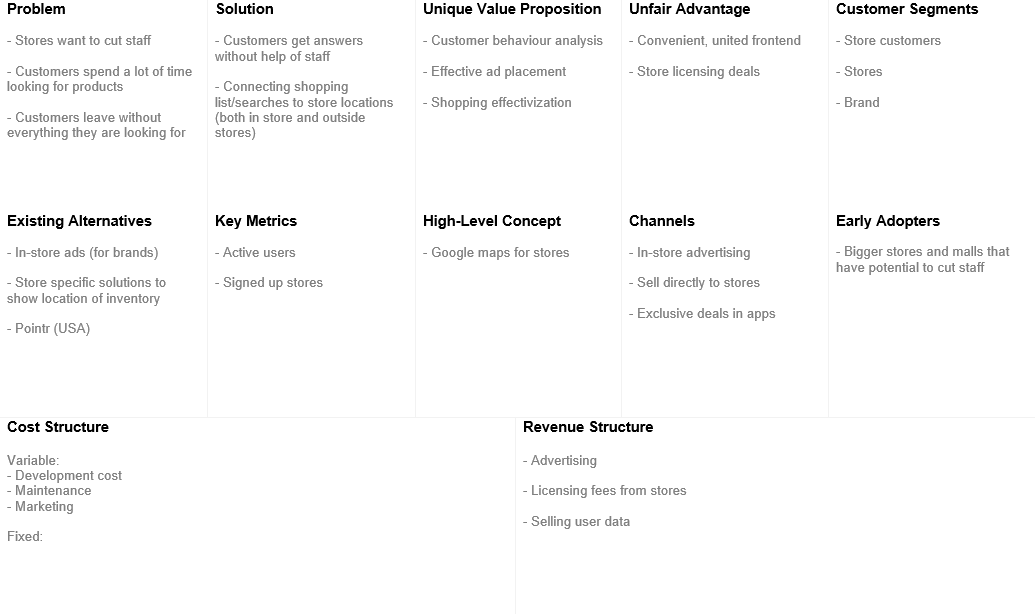
\includegraphics[width=1\textwidth]{lean model canvas.png}
    \caption{Lean model canvas describing \companyName's business model}
    \label{fig:lean-model-canvas}
\end{figure}

\subsection{MOM Testing and Prototyping} 

We used the mom test to understand potential users' experiences with in-store shopping in order to refine and validate our market-product fit. 
Friends, family and coworkers of team members were asked the following questions:
\begin{enumerate}
    \item How would you describe your in-store shopping habits?
    \item Do you regularly have issues navigating stores?
    \item How do you typically address these issues?
    \item Do you typically ask retail employees questions about item locations or current deals?
    \item Are there certain types of stores you avoid?
    \item What could persuade you to start shopping at these stores?
    \item Is it important for you to save time while shopping?
\end{enumerate}
Our small-scale research found that a majority of the people we asked were interested in cutting down the time it takes for them to shop, especially in grocery stores. It also suggested that users are not opposed to using digital tools to navigate within stores.
Many test subjects expressed frustration in regularly having issues finding certain items. Frustration was also described in not reliably being able to ask in-store personnel questions, either due to social barriers or more commonly due to lack of available personnel. 
The results from the test suggest that our solution fits well into the current market.

Prototyping provided further insights as our mockups, as seen in figure \ref{fig:mockups}, were presented to a new round of subjects. 
These insights were used to narrow down what features were most important to users and confirmed the validity of existing ideas, such as in-app ad space. 
Our product would directly address these issues perceived by the public. Unlike current solutions, which give minimal or no information to the consumer on where to go for various items,
our solution aims to instead give the consumer the ability to find items with a mobile solution,
letting them obtain information of product positions without having to actively seek them out.
In addition, the staff requirement of providing information to store customers would be greatly relaxed.

Usage and improvement of shmap are tightly interconnected, as our product can be improved over time by utilizing our users data, such as customers' store positions and user-provided complementary map data.
Unlike other solutions, our model can also combine the data from different model consumers, facilitating a high potential for growth.

\begin{figure}[h!]
    \centering
    \begin{subfigure}[b]{0.3\linewidth}
        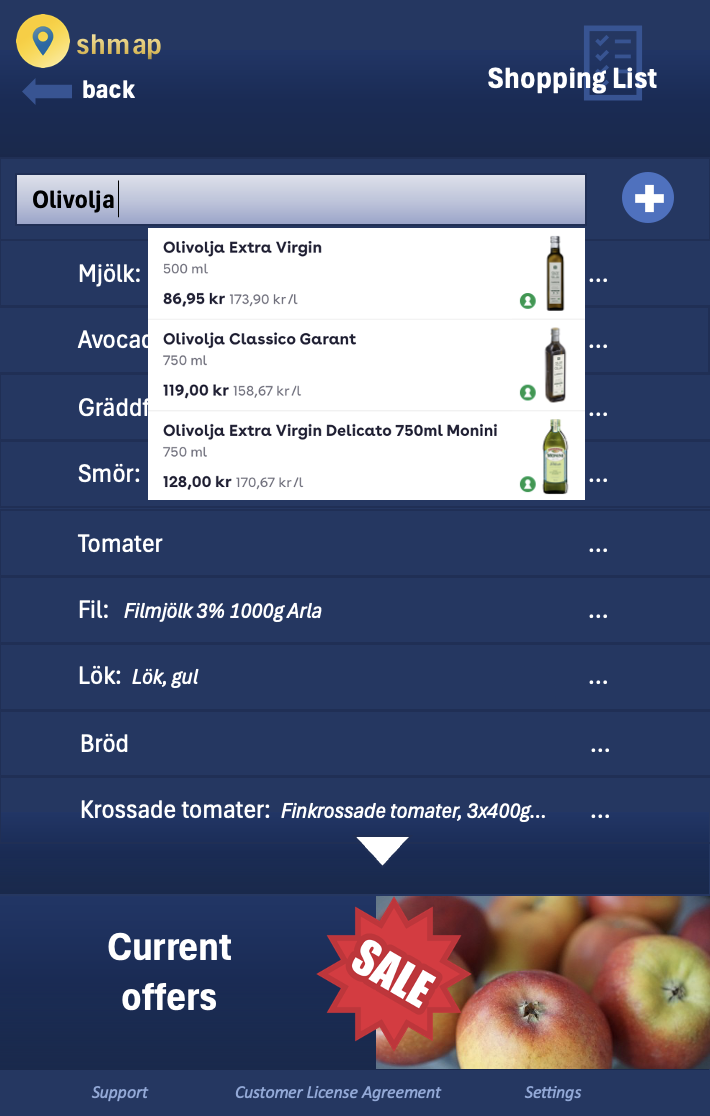
\includegraphics[width=\textwidth]{ShopList.png}
        \caption{Mockup of shopping list functionality}
      \end{subfigure}
      \begin{subfigure}[b]{0.3\linewidth}
        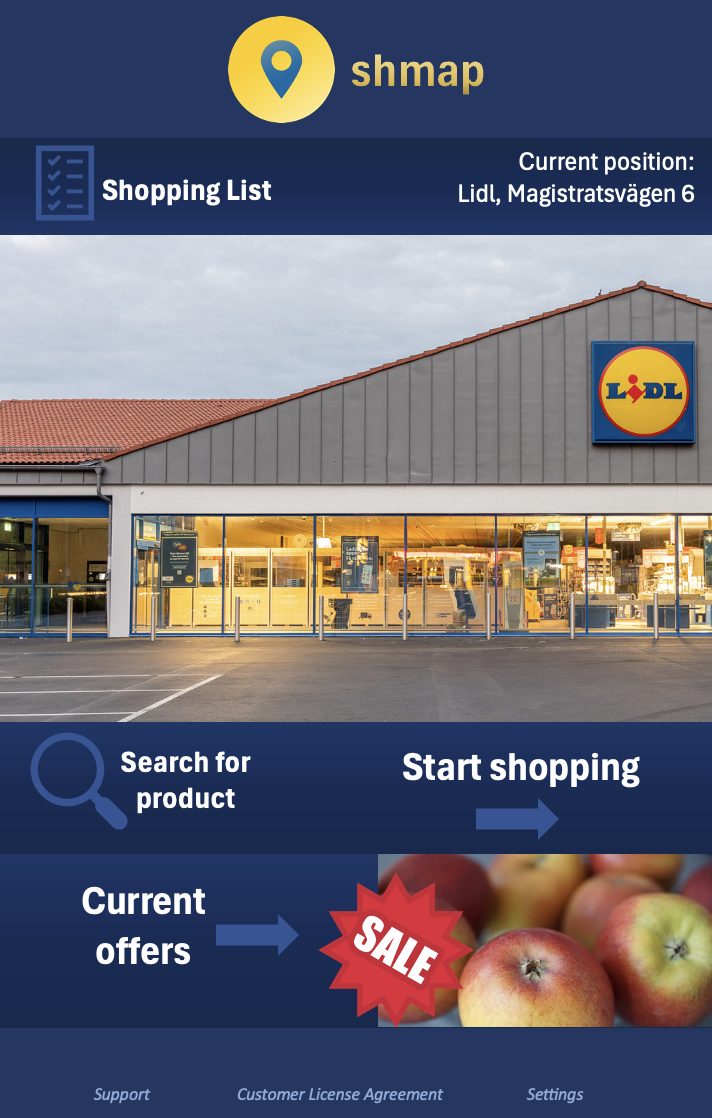
\includegraphics[width=\textwidth]{StoreHome.png}
    \caption{Mockup of a storefront page}
      \end{subfigure}
    \begin{subfigure}[b]{0.3\linewidth}
      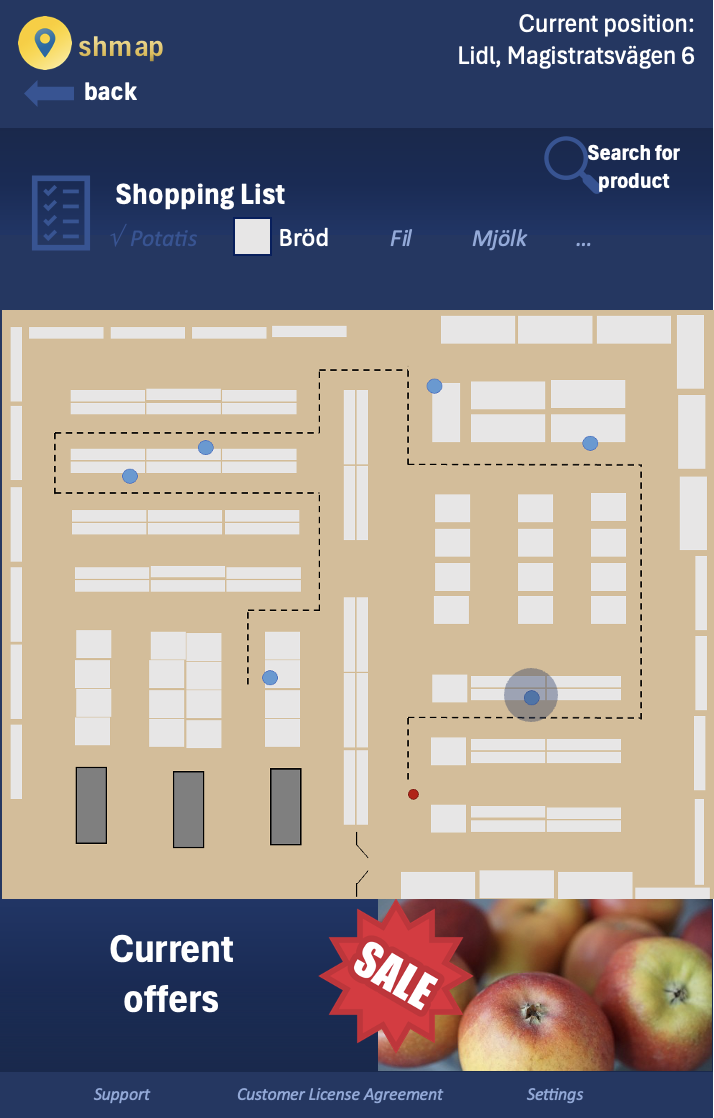
\includegraphics[width=\textwidth]{ShopRoute.png}
    \caption{Mockup of route navigation functionality}
      \end{subfigure}
    \caption{Three simple mockups}
    \label{fig:mockups}
\end{figure}

\subsection{Cost and Revenue Model development}

From the ideas that arose during the initial workshopping, our team worked to develop a concrete plan for both costs and revenue.

\subsection{Revenue Model}

It became clear to us that a sustainable business model for both our company and our clients would be a licensing fee, where a retail client pays a fee to implement their location into our product. 

An early challenge was identified in motivating potential customers, as we realised that retailers might be hesitant to pay to license a product that would lead to shoppers spending less time in stores.
This is due to the established correlation between spending time and spending money in stores \cite{byron}. To combat this theoretical reluctance, our team realised the value in providing analytic data of shopper movement within their locations. Retail stores spend large amounts of money yearly to optimize store layouts, but rely on more broad metrics such as purchases per shopper or shoppers per day.

With our unique data, retailers will gain unique and detailed insights into where their shoppers are spending time within stores, allowing them to create effective adjustments to layout and product placement.

Therefore, licensing our product would not only provide them the opportunity to cut labor costs on store personnel needing to assist shoppers with navigation and stock info, but also provide unique insights into shopper behavior. Our team feels that this proposition outweighs potential loss of user time spent in stores.

In addition to this, significant streams of revenue are to be gained from in-app advertisement. The value of providing users with context-appropriate ads related to things they are actively searching for is quite substantial, and we believe our product provides unique value to this area.

\subsection{Cost Model}

The team used preexisting knowledge and experiences of app development to develop a structure of variable and fixed costs:

\subsubsection{Fixed costs}

\begin{itemize}
  \item App Development and Maintenance:
  \begin{itemize}
    \item Salaries
    \item Design costs
    \item Testing tools and QA
  \end{itemize}
    \item Cloud/server infrastructure
    \item Third-party APIs for mapping and localization
    \item Office space (optional if remote first)
    \item Administrative costs
    \item Legal costs
  \end{itemize}
  \subsubsection{Variable costs}
  \begin{itemize}
    \item Digital advertising
    \item Content marketing
    \item Retailer outreach
    \item Customer support
  \end{itemize}

\section{Market Analysis}

Our product would be aimed at in-store shoppers, people who want help getting around different stores and getting the best possible deals for what they are searching for. There are multiple current alternatives that cover part of what we aim for. For example, many supermarket stores have their own apps that show weekly deals, searching for products, among other things. Other apps like Tiendeo offer the possibility of seeing the catalog of discounts in nearby stores in your area. And the stores themselves usually display their own discounts and offer physical catalogs with their offers. 

Though this helps when searching for deals, it does not help customers find their way within the store, where they would rely on looking around, checking the signs or asking for help from the store personnel. Pointr offers the possibility of indoor positioning, but it has not reached the Swedish market, and it is limited to countries like the US and the UK. 

We present a unique opportunity for companies that partner with us to collect data on in-store customer behaviour, especially when privacy laws are increasingly restrictive on what data companies can collect. By using the shopping list and the route that the customer takes throughout the store, we can track what items customers buy beyond what they initially intend to. This can help the stores improve their in-store marketing and figure out what gets the customer to stop in their tracks and spontaneously purchase an item.

From the purely technical perspective, our startup has the competency to develop an initial working prototype or something resembling a finished product. The main worries would be maintaining a larger operation and managing the legal side of the startup since we are a small team of computer science and engineering students.

Our product has the ability to combine the side of navigation within the store, optimizing routes according to items or shopping lists, plus promoting the user with deals and offering the option to compare product prices in different stores from the comfort of a single app.

For our initial market we would aim to partner with some individual stores in limited locations to show to both users and customers, like supermarket chains, the possibilities our app offers. We would start with a smaller city, like Lund, and promote the app in front of the stores we would be partnered with. We would aim our product mainly at bigger families, who want to optimize the time they spend in stores and the amount of money they spend on products.

Through the use of prototyping we were able to explore, on a small-scale, the viability of our product with its target audience. This was done using a general description of the product alongside the mock-up images, see Figure \ref{fig:mockups}.
This prototyping provided further insights, as potential users were allowed to visualize the product and results were largely positive. Valuable feedback in requests for functionality and accessibility provided our team with structure for implementing a final product.

A worry with our product is that initially it is up to the stores which we partner with to push the customers to use the product. Many customers get used to their own habits of shopping and would be reluctant to use a service with the intent of breaking their habits and making them visit other stores in order to get the best deals. Since we intend to work with convenience and retail stores who most likely have already established a customer base, it might be difficult to incentivize them to use a new system in order to better their customer experience with no guarantee that it will make a difference.

\subsection{SWOT}

As a group our technical competence is great and we have experience with startups, graphical design, working in grocery shops and programming. Since we are six computer science students we would be able to solve software issues which arise such as bugs and implementing features which customers request. We have made an accurate depiction of how our product would fit into the market and have come up with a great way to appeal to customers and how our product would solve issues perceived by the public.

\section{Implementation plan}

The launch of shmap hinges on its main features, navigation, product search and the shopping list, being implemented into a cohesive application. The system of anatomy of \companyName, as described in figure \ref{fig:sysanat}, allows us to structure a time-based implementation plan, which is shown in figure \ref{fig:ganttchart}.

\begin{figure}[h]
    \centering
    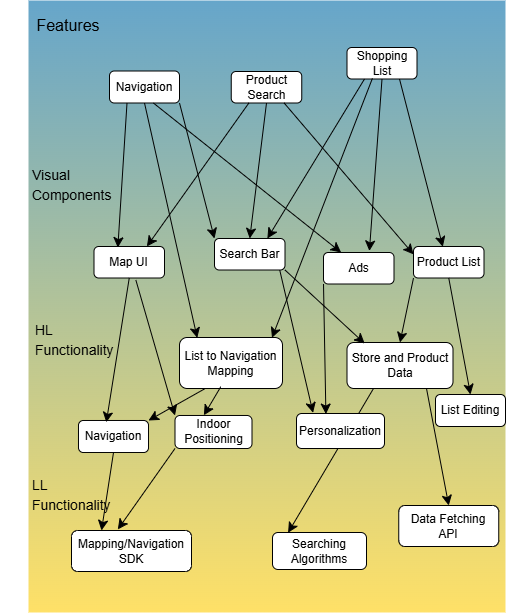
\includegraphics[width=0.5\textwidth]{SystemAnatomy.png}
    \caption{\companyName's system anatomy}
    \label{fig:sysanat}
\end{figure}

\begin{figure}[h]
    \centering
    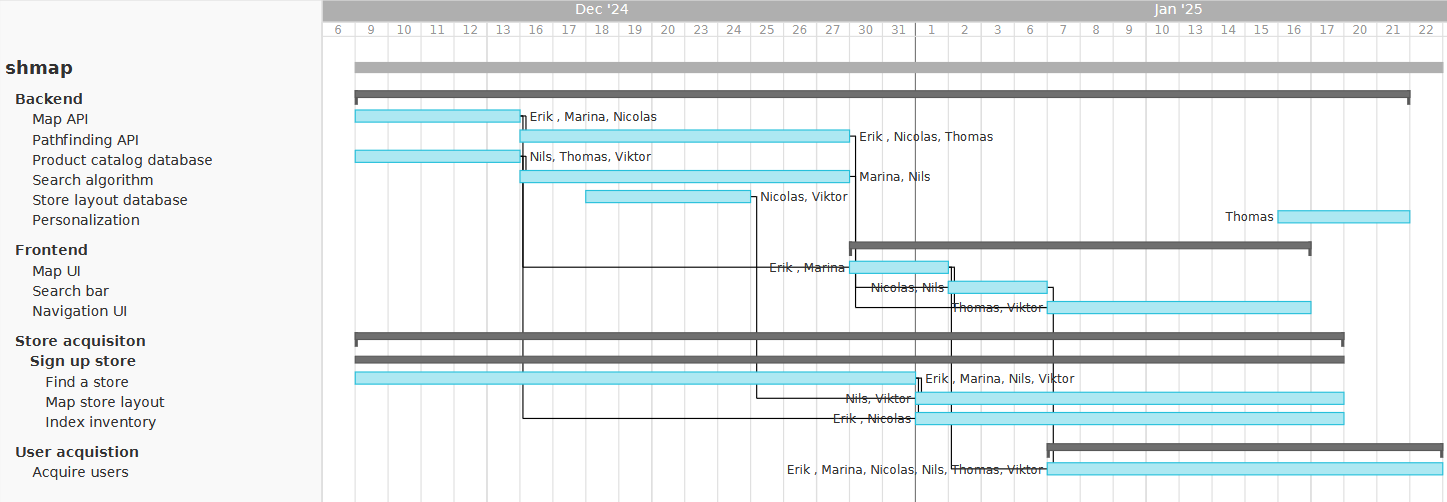
\includegraphics[width=1\textwidth]{implementation_plan.png}
    \caption{Gantt chart describing the implementation plan of \companyName}
    \label{fig:ganttchart}
\end{figure}




\section{Risk assessment}

A risk assessment of the entirety of this project concludes that significant risks stem from two sources: lack in interest from users and businesses, and risks associated with the inexperience of the team.

A failure to attract enough attention from and involvement of users in our product would make it significantly more difficult to attract investors as well as attract advertising companies, therefore directly affecting our main stream of revenue. Lacking interest from businesses will also make it difficult expand the usability of our product, in turn making it less desirable for users.

In order to mitigate these risks, MOM-tests and prototyping will help the team ensure that there is a market for the product, and that the problem-solution fit is good. Exclusive offers for partner businesses and users at the initial stages may help attract more of both categories. Prototyping at different stages in development, both for user side application and business side maintenance, to further solidify the solution is a good fit will help create a successful product. Offering help with setup and integration into existing warehouse management systems can help ease businesses who are concerned with the amount of work required, for set-up and maintenance alike. 

Inexperience in the team give rise to risks involving poor or insufficient planning, and an unrealistic schedule and budget. The plan may lack in granularity in turn leading to inaccurate estimates. Some important tasks may be overlooked or forgotten, or things may be planned out in a suboptimal way. Resources may be wrongly distributed causing a delay in some part of the project while an other part is stalled waiting for the delayed part.

By carefully applying well tested and known methods in creating a system anatomy and implementation plan, we hope to mitigate some of the risk. Methods like planning poker to estimate effort on different activities, and trying to give a little more slack than believed necessary would create some extra room for error. Regular check-ins with the team to see the progress will allow potential problems to be discovered earlier so that action may be taken to minimize consequences. If possible a mentor or a review by someone with more experience in software related business could also be helpful when finalizing the implementation plan.

A complete risk assessment, including risks, risk level estimation, mitigating actions and monitoring can be found in the table below.

\begin{center}
\footnotesize
\begin{longtable}{p{2.1cm}|p{3.5cm}p{1.2cm}p{3.5cm}p{1.7cm}}
\multicolumn{5}{c}{\bfseries Risk Assessment Table}\\
\\
\hline
\\
 Level & Specification & Risk est. & Mitigation & Monitoring \\
 \\
 \hline
 \\
User level & Low involvement of users. Not interested in new tech/solution, do not consider the "problem" substantial enough to want a solution for it. Not interested in learning how to use it. & medium & MOM-test. Prototyping to ensure simple, easy to use UI, good fit for the problem. Exclusive offers to attract customers. & Prototype to get feedback \\
\\
& Low interest from businesses. Perceive gains as small compared to work required. Not willing to learn new technology. & high & Prioritize simple and quick maintenance on business-end. Integration into their WMS. Prototyping. On site support to set up. Offer training to staff. & Prototype to get feedback \\  
\\
\hline
\\
Requirements gathering & Requirements not deliverable: cannot get precise enough indoor location services for mapping & low & Early testing. Adjust plan? Plan for alternative solution. & Research before starting implementation, alternative solution? \\
\\
& Misunderstood or incomplete requirements. Misunderstood MOM-test results, and prospective users expect something other than what we have in mind. Missing important requirement for users to adopt our solution. & low & Prototyping, feedback including ads. & Prototype to get feedback \\
\\
\hline
\\
Planning & Unrealistic schedule and budget, unrealistic goals. (Inexperienced team) & medium & Leave extra room. Planning poker to estimate effort for different activities. & Regular check-ins with time plan \\
\\
& Insufficient granularity in time plan. Missed or overlooked steps. & medium & SPM-tools to try and develop a more detailed plan to minimize risk of missing something important. Planning poker: if large variation in estimated effort, or large effort for a given task, perhaps a sign it can (should) be broken down further? & Regular check-ins with time plan \\
\\
\hline
\\
Analysis &  Faulty cost-benefit analysis: planned development of a minor feature turns out to be much more expensive than initially expected & low & Periodic revisions of the plan and re-prioritizing items. Using a fine granularity when planning to clarify what needs to get done. & Regular check-ins with time plan \\
\\
\hline
\\
Design &  Lack of integrity in design elements, bad or difficult to use UI & low & Perform prototyping to get user feedback on UI & Prototype tp get feedback \\
\\
&  Lack of proper architectural design and plan & low & Separate activity to plan proper architecture. Create structure documents, UML-diagrams, and design meetings with team to ensure everyone is on board. Document structure. & Periodic code reviews \\
\\
\hline
\\
Implementation &  Programming errors & low & Test first, clean branch with only working code to ensure no broken code contaminates the working space. Internal code reviews. & Periodic code reviews, continuous testing \\
\\
&  Lack of proper documentation and comments, difficult to understand for other team-members & low & Plan and create clear guidelines on documentation for produced code. Periodic internal code reviews. & Periodic code reviews \\
\\
&  Lack of necessary skills & low & Clear resource planning to ensure the best fit between resource and task. Team stand-up meetings to quickly discover if there is a problem, so that resources may be redistributed. & Team check-ins \\
\\
\hline
\\
Maintenance &  Lack of proper documentation & low & Clear guidelines on documentation. Internal code reviews regularly. & Periodic code reviews, continuous testing \\
\\
& Too complex for businesses to maintain: too involved, too much work, too difficult for staff & medium & Prototyping business side UI, get feedback on documentation, offer ongoing support. Already in planning stage plan for integration into existing WMS to minimize necessary effort from businesses to maintain. & Pre-release feedback \\
\\
& Political or legal changes that have a negative impact & low & Alternative ways of generating revenue if laws on gathering user data tightens for example & Monitor politics and news in relevant sector \\
\\
\hline
\label{risktable}
\end{longtable}
\normalsize
\end{center}

\section{Appendix}
\subsection{Contribution statement}
Thomas Dellwik: Part of group brainstorming and discussions when forming our business idea and MOM-test questions. Responsible for writing the Business model section in the first draft of the report. Spent around 5 hours total. \\
\\
Marina Fridh-Cardoso: Participated in discussions in regards to formulating and refining our business idea. Strengths and weaknesses, how to create value for both customers (retailers) and users. Active in planning and executing MOM-test. Together with team members filled out the Lean Canvas. Formalia and structure of report draft. Created prototypes. Made a risk assessment and wrote the corresponding section, and created the risk assessment table. Approx. 16 hrs of work total. \\
\\
Nicolas Jaua Otero: Active part in discussions and planning of business idea and strategy. Contributed to MOM-test planning and execution. Wrote the Market analysis section of the report. About 5 hrs work.\\
\\
Viktor Jernberg: Took part in brainstorming, refining and planning business idea and business strategy, following the Lean Canvas Model. Active part of planning and executing the MOM test. Responsible for writing first draft of Management team section. About 5 hours.\\
\\
Erik Nicander: Participated in group discussions and planning, attended seminars and group planning meetings. Took an active role in developing our business idea and in fleshing out the business strategy and filled in the Lean Canvas. Approximately 5 hours of work in total.\\
\\
Nils Reberg: Took on a leading role in coming up with and refining the business idea and strategy, and completing Lean Canvas.  Involved in planning and execution of MOM-test. Author of the Executive summary section. Total time about 5 hrs spent.\\

%\newpage
\bibliography{bibliography}
\bibliographystyle{unsrt}

\end{document}
